% Para compilar la primera vez que se agrega una referencia (/cite):
% Seguir estos cuatro pasos:
% latex Nombre-del-archivo.tex
% bibtex Nombre-del-archivo (sin el .tex)
% latex Nombre-del-archivo.tex
% latex Nombre-del-archivo.tex


% Etiquetas que uso para editar en la próxima iteración:
% FALTA, VER


\chapter{ \textsc{ Sumadores } }\label{diseñoDigital}
	
\section{Introducción}
Tal como mencionamos en la sección \ref{sec:intro_esp} (pág. \pageref{sec:intro_esp}), nuestro objetivo es implementar un sumador binario de $n$ bits, manteniendo la mejor relación de compromiso entre performance, potencia y área según crece \(n\).


% Selección de la Arquitectura 
\subsection{Selección de la arquitectura}\label{sec:selección_arquitectura}

Se puede afirmar que los sumadores llamados (según la bibliografía en inglés) como \emph{parallel prefix adders}\footnote{Nosotros los nombraremos como \cursi{sumadores de prefijo paralelo}.} son los mejores con respecto al producto potencia-retardo\footnote{Cuando decimos retardo, nos referimos al retardo de propagación máximo de un circuito, nuestra métrica elegida para caracterizar la performance.}.  Estos sumadores se clasifican dentro de un mismo tipo, porque reducen el problema de calcular las señales de acarreo como el \textbf{problema de cálculo de prefijo}\footnote{En \ref{subsec:prefixProblem} definimos precisamente el problema.}. A su vez, son implementaciones particulares de los sumadores  conocidos como \emph{carry look-ahead adders}, ya que todos se basan en el cálculo en paralelo de los acarreos.
\subsubsection{\emph{Sumadores de prefijo paralelo}}
Brent-Kung\cite{brent-kung}, Sklansky\cite{sklansky}, Kogge-Stone \cite{kogge-stone}, Ladner-Fisher\cite{ladner-fischer}, Hans-Carlson\cite{kogge-stone} y Knowles\cite{knowles} son implementaciones de este tipo de sumadores, que se diferencian cada uno por minimizar alguna relación de compromiso, en el espacio de diseño para el retardo, área y potencia\cite{Sugla-Carlson} del circuito.

Si tenemos en cuenta el área utilizada por estos circuitos, no podemos asegurar que una de estas se clasifique globalmente como la mejor, ya que algunas implementaciones favorecen una métrica a costa de la otra. Citamos un estudio que presenta los siguientes resultados de la figuras \ref{retardo-bits} y \ref{area-bits} de un estudio comparativo \cite{estrada-gimenez} para tecnología CMOS 0.13~\microm.

\subsubsection{Arquitecturas a implementar}
De estas arquitecturas mencionadas, vamos a implementar un sumador rápido basado en la idea original de Sklansky\cite{sklansky} publicado en 1960. También vamos a implementar una arquitectura que busca la mejor relación entre interconexiones y cantidad de compuertas utilizadas, a costa de un pequeño aumento en la cantidad de etapas, conocido como sumador de Brent-Kung\cite{brent-kung}. Además, implementaremos el sumador de ripple carry para utilizarlo de referencia comparativa.


\begin{figure}[h]
  \centering
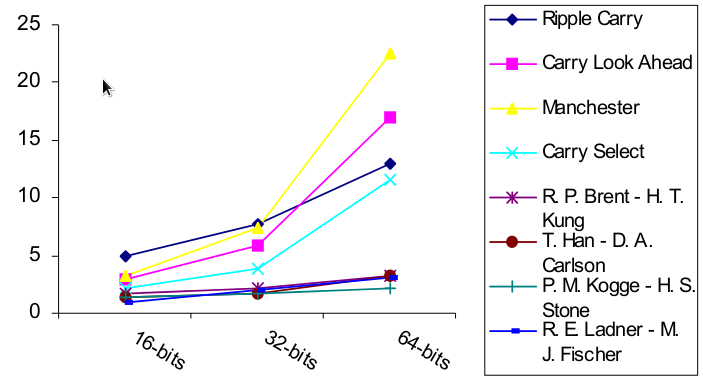
\includegraphics[scale=0.49]{figuras/retardo-bits.png}
\vspace{-5pt}
  \caption{Retardo respecto al tamaño de los operandos}
  \label{retardo-bits}
\vspace{-5pt}
\end{figure}


\begin{figure}[h]
  \centering
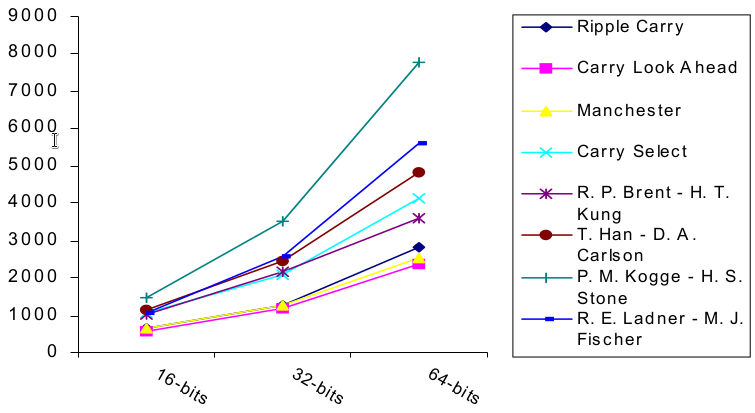
\includegraphics[scale=0.44]{figuras/area-bits.png}
\vspace{-1pt}
  \caption{Área respecto al tamaño de los operandos}
  \label{area-bits}
\vspace{-15pt}
\end{figure}

\begin{table}[h]
\centering
\begin{tabular}{|l|l|l|}
\hline
\multicolumn{1}{|c|}{\textbf{Arquitectura}} & \multicolumn{1}{c|}{\textbf{Retardo Máx.   }} & \multicolumn{1}{c|}{\textbf{Área}} \\ \hline
Ripple Carry  & \(O(n)\) & \(O(n)\) \\ \hline
Carry Look-Ahead  & \(O(\log(n))\) & \(O(n\log(n))\) \\ \hline
Ladner-Fisher &\( O(\log_2(n))\) & \(O(n\log(n))   \) \\ \hline
Sklansky &\( O(\log_2(n))\) & \(O(n\log^2(n))\) \\ \hline
Kogge-Stone & \( O(\log_2(n))\) & \\ \hline
Han-Carlson &... &... \\ \hline 
Brent-Kung & $O(\log_2(n))$ & \(O(n\log_2(n))\) \\ \hline
\end{tabular}
\caption{Resumen de las funciones de retardo y área algunos sumadores}\label{tabla:sumadores}
\end{table}
Resumimos en la tabla \ref{tabla:sumadores} las características y diferencias entre los distintos sumadores\cite{6120598}. Incluimos al \textbf{ripple carry}, por ser la implementación más simple, y al \textbf{carry look-ahead} por ser el sumador que propone el cálculo en paralelo de los acarreos para disminuir logarítmicamente el tiempo de retardo.

%Agregar las referencias a los papers si se puede

%Para justificar la tabla de arriba, vemos los siguientes dos papers:

%"A unified Adder Design" - Wang, Parhi.

%CARACTERIZACIÓN DE SUMADORES EN TECNOLOGÍAS FUERTEMENTE SUBMICRÓNICAS -  Adrián Estrada, Carlos J. Jiménez, Manuel Valencia



\section{Fundamentos teóricos de la suma}
A los fines de poder implementar estos sumadores, desarrollaremos las ecuaciones que nos permitan llegar a la descripción del \cursi{hardware}.

\subsection{Semisumador y sumador completo}
\subsubsection{Semisumador}
El {\bf Semisumador} (Half-adder) recibe 2 bits de entradas \(a\) y \(b\) y produce un bit de suma \(s\) y un bit de acarreo \(c\).

\begin{subequations}
\begin{align}
s &= a \oplus b\\
c &= ab
\end{align}
\end{subequations}

\subsubsection{Sumador Completo}
Luego definimos un Sumador Completo de un bit, o Full Adder:
\begin{center}
\begin{tabular}{lll}
Entradas: & Bits de operandos \(a\) , \(b\) y carry-in \(c_{in}\) & (o \(a_i, b_i, c_i\) para la etapa \(i\)) \\
Salidas: & Suma \(s\) y carry-out \(c_{out}\) & (o \(s_i\) y \(c_{i+1}\) para la etapa \(i\)) \\
\end{tabular}
\end{center}

\begin{subequations}
\begin{align}
s &= a\oplus b \oplus c_{in}
\label{s}
\\
c_{out}&= a b + a c_{in} + b c_{in}
\label{c}
\end{align}
\end{subequations}
%\(c_{out}= (a\wedge b )\vee (a \wedge c_{in}) \vee (b\wedge c_{in})\)

Podemos construir un {\bf sumador completo} (full-adder) combinando las ecuaciones del sumador y semisumador, como vemos en la figura \ref{fig:fulladder}:

\vspace{-1pt}

\begin{figure}[h]
  \centering
\hspace{-23pt}
\begin{subfigure}[b]{0.3\textwidth}
                \centering
                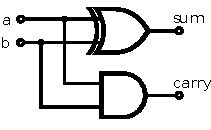
\includegraphics[width=\textwidth]{figuras/halfadd_schem.pdf}
                \caption{Semisumador}
                \label{fig:halfadder}
        \end{subfigure}
\begin{subfigure}[b]{0.5\textwidth}
                \centering
                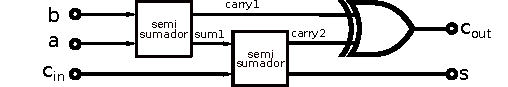
\includegraphics[scale=1.3]{figuras/fullAdd_schem.pdf}
                \caption{Sumador completo}
                \label{fig:fulladder}
        \end{subfigure}

  \caption{Bit adders}\label{fig:bitadders}

\end{figure}

\vspace{0.5cm}

%\section{Selección de la arquitectura del sumador}
%Proponemos el uso de Celdas estándard CMOS (Complementary Metal Oxide Silicon) para la implementación\footnote{Para ver otras posibilidades de implementación lógica, ver (FALTA CITA) RABAEY}. El carácter de nuestro flujo de diseño así lo requiere, ya que se utilizarán herramientas de síntesis de circuitos digitales basadas en celdas estándars. Quedan entonces descartadas las implementaciones utilizando transmition gates, lógica dinámica u otro tipo de implementacion lógica.

\subsubsection{Ripple Carry Adder}

Definimos el sumador Ripple Carry Adder (RCA), utilizando \(n\) sumadores completos para sumar 2 operandos de \(n\) bits. El sumador de \(n\) bits produce una salida de \(n\) bits y una salida de acarreo \(c_{out}\).

Este sumador se implementa conectando como muestra la figura \ref{fig:RCA} el bloque \verb.fullAdd. (Sumador Completo). El camino crítico de la señal se determina considerando el peor camino de propagación de la señal.  

%\vspace{-1pt}
\begin{figure}[h]
  \centering
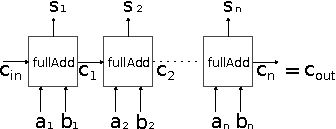
\includegraphics[scale=1.5]{figuras/binnaryAdder.pdf}
  \caption{Ripple Carry Adder}
  \label{fig:RCA}
\end{figure}

El retardo del camino crítico de un sumador de $n$ bits es:

\begin{equation}
T_{RCA} = (n-1)T_m+ T_{FA}
\end{equation}

Siendo $T_m$ el retardo del circuito de generación del acarreo de un sumador completo y $T_{FA}$ el retardo de un sumador completo. Es decir, el retardo es proporcional al tamaño de los operandos.

%\cite{estrada-gimenez}
%Comenzamos con el RCA (Ripple Carry Adder), que tiene un área O(n) y un retardo de compuerta (Delay) de O(n).
%Luego tenemos al CLA (Carry Look-Ahead Adder) con un área de O(n*log(n)) y un delay de O(log(n)).
%Carry Skip Adder(CSA)
%Carry Increment Adder (CIA) Área O(n) y Delay O (nl + 2/ l +1 )  
%Carry Select Adder (CSelA)Área O(n) y Delay O (nl + 2/ l +1 ) 
 
% El delay de un RCA está en pag. 77 de Computer Arithmetic de Behrooz Parhami

\subsection{Sumadores \cursi{carry lookahead}}

La clave para sumar rápido es plantear el problema de la suma como el problema de generar las señales de acarreo en el menor tiempo posible; eso queda evidenciado al interpretar la ecuación \ref{s_i}. Por lo tanto, el objetivo será lograr un bloque generador de las señales de acarreo de baja latencia\cite{arithmeticComputer}.
%Pag. 85 - Section 5.6 (ver como se cita en latex la página)

Ya que una vez que el acarreo en la posición \(i\) es conocido, se puede calcular la suma como:
\begin{equation}\label{s_i}
s_i = a_i \oplus b_i\oplus c_i
\end{equation}

Con respecto al acarreo, lo importante es si en una posición dada el acarreo se \emph{genera} ó se \emph{propaga}. Con las siguientes ecuaciones lógicas podemos definir esas señales:
%

%\vee es el OR
%\wedge es el AND
%\oplus es el XOR
%$$a_i=\lnot{a_i}\wedge\lnot{b_i}=\lnot{(a_i \vee b_i)}$$
$$g_i=a_ib_i$$
$$p_i=a_i \oplus b_i$$


Asumiendo que estas señales se han calculado y están disponibles, podemos calcular recursivamente el acarreo de la siguiente forma:
\begin{equation}
%c_{i+1}=g_i\vee (c_i \wedge p_i)
c_{i+1}=g_i + c_i p_i
\end{equation}


\noindent Esto quiere decir que un acarreo entrará en la etapa \(i+1\) si éste se genera en la etapa \(i\), o si entra en la etapa \(i\) y se propaga.

\subsection{Desenrollando la recurrencia del acarreo}
Uno puede desenrollar esta fórmula recursiva del acarreo hasta lograr una función que dependa directamente de los operandos ($a$ y $b$) y del acarreo de entrada $c_{\text{in}}$:
\begin{equation}
\begin{align}
c_i &= g_{i-1} + p_{i-1}c_{i-1}\notag\\
&=g_{i-1}+p_{i-1}(g_{i-2}+p_{i-2}c_{i-2})=g_{i-1}+p_{i-1}g_{i-2}+p_{i-1}p_{i-2}c_{i-2}\notag\\
&=g_{i-1} + p_{i-1}g_{i-2}+p_{i-1}p_{i-2}g_{i-3}+p_{i-1}p_{i-2}p_{i-3}c_{i-3}\notag\\
&=g_{i-1} +p_{i-1}g_{i-2}+p_{i-1}p_{i-2}g_{i-3}+p_{i-1}p_{i-2}p_{i-3}g_{i-4}+p_{i-1}p_{i-2}p_{i-3}p_{i-4}c_{i-4}\label{gyp}	
\end{align}
\end{equation}

El proceso se repite hasta que el último término contenga $c_0 = c_{\text{in}}$. Podemos computar todos los acarreos en un sumador de $k$-bit directamente con las señales auxiliares ($g_i,p_i$) y $c_{\text{in}}$, utilizando compuertas lógicas AND-OR con un fan-in máximo de $k+1$. Para $k=4$, tenemos:
\begin{equation}
\begin{align}
c_4 &=g_{3} +p_{3}g_{2}+p_{3}p_{2}g_{1}+p_{3}p_{2}p_{1}g_{0}+p_{3}p_{2}p_{1}p_{0}c_{0}\\
c_3 &=g_{2} +p_{2}g_{1}+p_{2}p_{1}g_{0}+p_2p_1p_0c_0\\
c_2 &=g_{1} +p_{1}g_{0}+p_{1}p_{0}c_{0}\\
c_1 &=g_0+p_0c_0\\
\label{carries}	
\end{align}
\end{equation}	
Aquí, $c_4$ y $c_0$ son los $c_{\text{out}}$ y $c_{\text{in}}$ respectivamente de un sumador de 4-bits. Podemos usar un bloque de acarreo basado en estas ecuaciones, y usando compuertas AND de 2 entradas para $g_i$ y compuertas XOR de 2 entradas para $p_i$ y los bits de suma, construimos un sumador de 4-bits. Este sumador es conocido como \emph{carry lookahead adder (CLA)}. Notar que como $c_4$ no se usa para calcular la suma, no es necesario aplicar la ecuación \ref{carries} y lo podemos obtener usando una ecuación más simple, sin tener casi un deterioro en velocidad:
\begin{equation}
\begin{align}
c_4 = g_3 + c_3p_3 \notag
\end{align}
\end{equation}
La red de acarreo que resulta de estas ecuaciones la podemos ver en la figura \ref{cla4bits}.
\begin{figure}[h]
  \centering
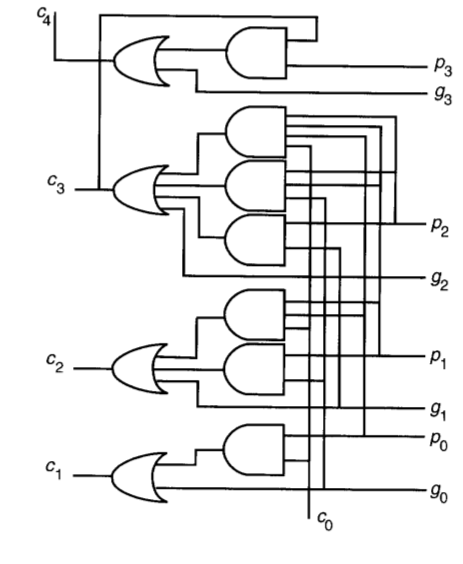
\includegraphics[scale=0.43]{figuras/fulladder4bitcla.png}
\vspace{-1pt}
  \caption{CLA 4-bits}
  \label{cla4bits}
\vspace{-15pt}
\end{figure}

Si observamos las ecuaciones \ref{carries}, vemos que el retardo de esta red será el retardo $T_{AND_n}$ de la mayor celda AND, mas el retardo $T_{OR_n}$ de la operación OR de $n$ entradas. Esto es un inconveniente, ya que según aumenta el fan-in también aumenta el retardo. El retardo de un sumador construido con esta red tendrá también el retardo $T_p$ del cálculo de $p$ mas el retardo de un sumador completo.
\begin{equation}
T_{CLA} = T_p + T_{AND_n} + T_{OR_n} + T_{FA}
\end{equation}

Se pueden realizar por medio de árboles binarios una reducción a celdas con un fan-in de dos (por ejemplo), pero agregando una etapa por cada reducción, en ese caso el retardo en este circuito sería en función del $\log_2 n$.


% INTERESANTE: Clock periods in contemporary microprocessors are rather short; they are shorter than 10 times the delay of a full-adder.

\subsection{Sumadores de Prefijo Paralelos (\emph{Parallel Prefix Adders})}
En la sección anterior vimos como desarrollar ecuaciones que nos permiten obtener las señales de acarreo a partir de las señales auxiliares, para poder calcular la suma del bit $n$, sin esperar a que el acarreo del bit $n-1$ sea computado. Aunque esta solución tal cuál como la presentamos deja de ser aplicable según aumenta $n$, nos permite abordar \textbf{el problema del cálculo de los acarreos como un problema de prefijo paralelo}.
\subsubsection{Problema de prefijo paralelo (\emph{parallel prefix problem})}\label{subsec:prefixProblem}
El problema de prefijo paralelo es:

\begin{equation}
\begin{align}
\text{Dado:}\\
 & \text{Entradas:} x_0,x_1,\dotsc,x_{k-1} \\
 & \text{Un operador + asociativo}\\ 
\text{Computar}:&x_0 \nonumber \\
&x_0+x_1 \nonumber \\ 
&x_0+x_1+x_2+ \nonumber \\ 
&\vdots \nonumber \\ 
&x_0+x_1+x_2+\dotsb+x_{k-1} \nonumber
\end{align}
\end{equation}

\subsubsection{Cómputo del acarreo como un problema de prefijo paralelo}
Pensemos la ecuación \ref{gyp} de la siguiente forma, asumiendo que $c_0=c_\text{in}$ viene desde otro bloque:
\begin{equation}
\begin{align}
g_{[i,i+3]} &= g_{i+3}+g_{i+2}p_{i+3}+g_{i+1}p_{i+2}p_{i+3}+g_{i}p_{i+1}p_{i+2}p_{i+3}\nonumber\\
p_{[i,i+3]} &= p_{i}p_{i+1}p_{i+2}p_{i+3}\nonumber
\end{align}
\end{equation}

Podemos interpretar estas ecuaciones de la siguiente forma: las cuatro posiciones de bits propagan colectivamente un acarreo $c_\text{in}$ si y solo sí cada una de las posiciones propaga; y el bloque gener	a un acarreo si en la posición $i+3$ se genera uno, o se podrouce en la posición $i+2$ y es propagado por la posición $i+3$, etc.

Con este procedimiento podemos llegar a expresar una generalización muy importante, para bloques adyacentes que se superponen $[i_1,j_i]$ y $[i_0,j_0]$, con $i_0 \leq i_1 - 1 \leq j_0 < j_i $:
\begin{equation}
\begin{align}
g_{[i_0,j_1]} &= g_{[i_1,j_1]}+g_{[i_0,j_0]}p_{[i_1,j_1]} \nonumber\\
p_{[i_0,i_1]} &= p_{[i_0,j_0]}p_{[i_1,j_1]}\nonumber
\end{align}
\end{equation}
Aquí, $g_{[i_0,j_1]}$ y $p_{[i_0,i_1]}$ son las señales que producimos de 2 bloques adyacentes ($B''$ y $B'$ con sus señales asociadas $(g'',p'')$ y $(g',p')$) que para simplificar la notación nos permite reescribir la anterior ecuación como:
\begin{equation}
\begin{align}
g &= g'' + g'p''\nonumber\\
p &= p'p''\nonumber
\end{align}
\end{equation}
Ahora entonces definimos un operador acarreo $\circ$ para condensar estas operaciones:
\begin{equation}
\begin{align}
(g,p) &= (g'',p'') \circ (g',p') = (g'' + g'p', p'p'')\nonumber
\end{align}
\end{equation}
Este operador es un operador asociativo, y esto se puede demostrar utilizando la propiedad asociativa de los operadores OR y AND. Finalmente, ya tenemos un operador asociativo, y las entradas $(g''',p''')$,$(g'',p'')$,$(g',p'),\ldots$ que nos permiten plantear el problema de la construcción de la red (o bloque) de acarreos, como un \emph{problema de prefijo paralelo}:
\begin{equation}\label{eq:ppProblem}
\begin{align}
\text{Dados:}\\
 & \text{Entradas:} (g_0,p_0),(g_1,p_1),\dotsc,(g_{k-1},p_{k-1}) \\
 & \text{Un operador} \circ \text{asociativo}\\ 
\text{Computar}:\\
(G_0,P_0) = &(g_{[0,0]},p_{[0,0]})\\
(G_1,P_1) = &(g_{[0,0]},p_{[0,0]})\circ(g_{[0,1]},p_{[0,1]})\\
&\vdots  \\
(G_{k-1},P_{k-1}) = &(g_{[0,0]},p_{[0,0]})\circ(g_{[0,1]},p_{[0,1]})\circ \dotsc \circ(g_{[0,k-2]},p_{[0,k-2]})\circ(g_{[0,k-1]},p_{[0,k-1]})
\end{align}
\end{equation}
Retomando la ecuación \ref{s_i} de la suma, y con estas ecuaciones que nos dan las señales propagadas o generadas del acarreo, podemos construir distintos sumadores, que varían en la red de cálculo del acarreo, particularmente en cómo se elija la asociación del operador \cursi{acarreo} (a veces también mencionado como \cursi{operador punto}). La implementación mas básica (y lenta) sería la de ir asociando en serie a este operador, como vemos en la figura \ref{fig:ppserie}. Todos los sumadores de prefijo paralelo se diferencian escencialmente en la forma de asociar.
\begin{figure}[h!]
  \centering
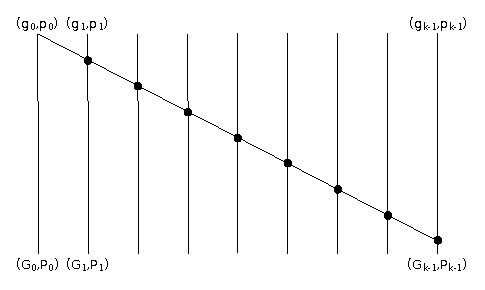
\includegraphics[scale=1.4]{figuras/ppserie.eps}
  \caption{Red de prefijo en serie, una forma gráfica de ver la ecuaciones del cálculo prefijo en \ref{eq:ppProblem}. Notar que cada línea representa dos bits. Los puntos negros representan al operador acarreo.}
\label{fig:ppserie}
%\vspace{-10pt}
\end{figure}
%118 del Parhami " Computer Arithmetic: Algorithms and Hardware Designs."



\subsection {Sumador de Brent-Kung}
Para tener en cuenta el problema de la interconexión entre las compuertas de forma tal que estas sean mínimas y que el área de celdas y de conexión se minimicen, se propone el sumador de Brent-Kung\cite{brent-kung}. Este sumador es una versión que considera el problema de la interconexión entre las compuertas, de una forma que minimice el área, a costa de un aumento en el retardo. Esto se expresa en la función de retardo que es \(2\log_2(n)-2\), a diferencia de los sumadores de Ladner-Fisher\cite{ladner-fischer}, Kugge-Stone\cite{kogge-stone} y Sklansky\cite{sklansky} que en \(\log_2(n)\) etapas calculan todas las señales de acarreo. 


\subsubsection {Operador de Brent-Kung}
El operador $\circ$ se define\footnote{Para respetar la notación de la bibliografía original comenzamos a utilizar la notación lógica con \(\vee\), \(\wedge\) y \(\oplus\) como los operadores booleanos AND, OR y XOR respectivamente} como:
\begin{equation}
(g,p) \circ (\hat{g},\hat{p}) = (g\vee(p\wedge\hat{g}),p\wedge\hat{g})\label{gap}
\end{equation}

\begin{figure}[h!]
  \centering
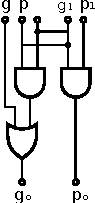
\includegraphics[scale=1.0]{figuras/dotOp_schem.pdf}
%\vspace{-5pt}
  \caption{Operator Punto de Brent-Kung}
  \label{dotOp}
%\vspace{-15pt}
\end{figure}
El operador Punto de Brent-Kung es asociativo, es decir:
$$((a,b) \circ( c,d))\circ (e,f)  = (a,b)\circ((c,d)\circ(e,f))$$
Y por lo tanto podemos ahorrarnos los paréntesis y escribimos:
$$(a,b)\circ(c,d)\circ(e,f)\circ...$$

\subsubsection {Circuito de Generación y Propagación de acarreo}
Ahora necesitamos un circuito que con cada bit de entrada de los operandos \(a\) y \(b\) calcule la señal de acarreo y la de propagación:
$$g_i=a_i \wedge b_i, p_i=a_i\oplus b_i$$
Esas señales se generan en paralelo, dado dos números binarios \(a[n]\) and \(b[n]\) de longitud \(n\).

%vspace{-10pt}

\begin{figure}[h!]
  \centering
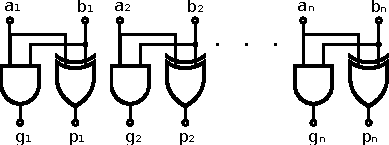
\includegraphics[scale=1]{figuras/gAndPs_schem.pdf}
  \caption{Generación y Propagación del Acarreo}
  \label{gAndPs}
\end{figure}

\subsubsection {Red de Prefijo Paralelo}
\noindent Con la figura \ref{bKung16}, detallamos ahora la red de prefijo paralelo con un fan-out máximo de dos, lo cuál diferencia a el sumador de Brent-Kung de los otros sumadores de prefijo paralelo. La red se realiza con 2 elementos: Los puntos negros son los operadores punto de Brent-Kung de la figura \ref{dotOp} y con buffers (los puntos blancos) que realizan una copia de la señal. Cada cable representa un par de bit \(g_i\),\(p_i\) de la figura \ref{fig:bkungadder}.

\subsubsection {Circuito completo}
Con la red de prefijo paralelo lista, podemos armar el circuito propuesto en el paper de Brent-Kung\cite{brent-kung}. A los fines de la implementación en HDL, mostramos el circuito visto de una forma alternativa en la figura \ref{fig:bkungadder}. Pero aprovechamos la oportunidad para generalizar un poco este resultado. Si retomamos la definición de la suma planteada en la ecuación \ref{s_i}:
$$
s_i = a_i \oplus b_i\oplus c_i
$$
y notamos que en la figura \ref{fig:bkungadder} se calcula $a_i \oplus b_i$, y que con los $G_i$ y los $p_{i-1}$ podemos construir la suma. Por lo tanto, no importa de qué forma se generen estas señales en la red de prefijo paralelo, podemos calcular el valor de $s_i$, como vemos de forma más genérica en la figura \ref{fig:ppadder}.

\begin{figure}[h]
  \centering
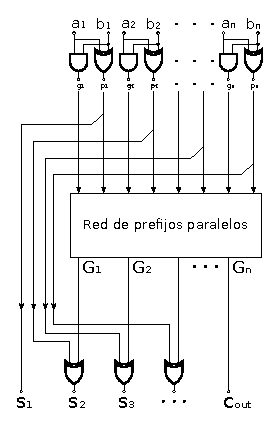
\includegraphics[scale=1.5]{figuras/arquitectura_schem_generico.eps}
  \caption{Sumador de prefijo paralelo}
  \label{fig:ppadder}
\end{figure}

\begin{figure}[h!]
\vspace{-5pt}
  \centering
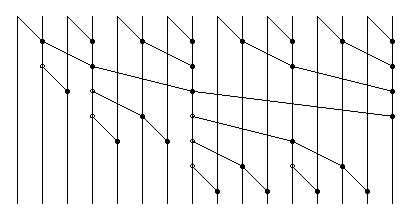
\includegraphics[scale=1.4]{figuras/bKung16.eps}
  \caption{Red de prefijo paralelo para Brent-Kung (ejemplo de 16 bits)}
\label{bKung16}
\vspace{-10pt}
\end{figure}

\begin{figure}[h]
  \centering
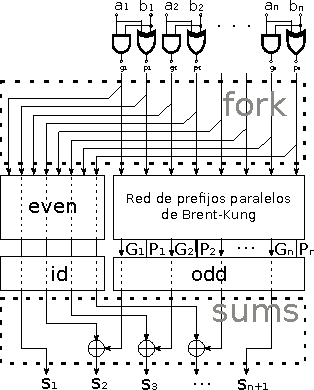
\includegraphics[scale=1.5]{figuras/arquitectura_schem.pdf}
  \caption{Sumador de Brent-Kung}
  \label{fig:bkungadder}
\end{figure}

\subsection{Sumador de Sklansky}\label{subsec:sklansky}
Para realizar este sumador, debemos desarrollar la red de cálculo paralelo de los acarreos, a la forma propuesta por Skalansky. Esta forma se conoce como \emph{divide and conquer}, y la evidenciamos con un ejemplo para sumandos de 16 bits en la figura \ref{fig:sklansky16}. Los puntos negros representan el operador punto (definido anteriormente como el operador de Brent-Kung), notar que tiene menos cantidad de etapas de operaciones (en proporción de $\log_2(n))$) por lo tanto es un sumador más rápido que el de Brent-Kung, pero hay nodos que tienen un fan-out de hasta $\frac{n}{2}$, lo cuál resulta en mayor capacidades parásitas, haciendo más lento el circuito en ese nodo.

\begin{figure}[h!]
\vspace{-5pt}
  \centering
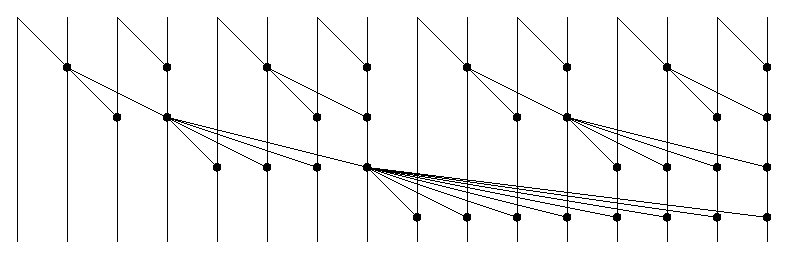
\includegraphics[scale=0.7]{figuras/sklansky16.eps}
  \caption{Red de prefijo paralelo para Sklansky (ejemplo de 16 bits)}
\label{fig:sklansky16}
\vspace{-10pt}
\end{figure}
